\documentclass{beamer}

\mode<presentation> {
  \usetheme{PaloAlto}
}

%%
\makeatletter
\setbeamertemplate{subsubsection in sidebar}{\vspace*{-\baselineskip}}
\setbeamertemplate{subsubsection in sidebar shaded}{\vspace*{-\baselineskip}}
\makeatother
%%

%%
\setbeamertemplate{theorems}[numbered]
%%

\definecolor{Garnet}{RGB}{130,0,20}
\usecolortheme[named=Garnet]{structure}

\logo{
\includegraphics[width=1.5cm]{../../sharedImgs/USClogo.png}}

%\setbeamercolor{title}{fg=red!60!black,bg=white!50!black}
%\usecolortheme{beaver}
%\usecolortheme{crane}
\usefonttheme{structuresmallcapsserif}
\usefonttheme[onlysmall]{structurebold}

\usepackage{multicol}
\usepackage{graphicx}
\usepackage{mathtools}
\usepackage{latexsym}
\usepackage{amsfonts}
\usepackage[only,ninrm,elvrm,twlrm,sixrm,egtrm,tenrm]{rawfonts}
\usepackage{indentfirst}
\usepackage[noend]{algorithmic}
\usepackage{algorithm}
\usepackage{enumerate}
\usepackage{graphicx,psfrag}
\usepackage{epsfig}
%\usepackage[pdflatex]{graphicx}
%\usepackage{epstopdf}
\usepackage{ulem}
\usepackage{animate} %need the animate.sty file
\usepackage{tikz}
\usetikzlibrary{fit,shapes,calc}
\usepackage{pgfplots}
\usepackage{amsmath,amsthm,amssymb,amsfonts,enumerate,mymath,mathtools,tikz-cd,mathrsfs}

\newtheorem{thm}{Theorem}
\newtheorem{lem}{Lemma}
\newtheorem{prop}{Proposition}
\theoremstyle{definition}
\newtheorem{defn}{Definition}
\newtheorem{rmk}{Remark}

\newcommand{\A}{\mathscr{A}}
\renewcommand{\C}{\mathscr{C}}

\newcommand*{\defeq}{\mathrel{\vcenter{\baselineskip0.5ex \lineskiplimit0pt
                     \hbox{\scriptsize.}\hbox{\scriptsize.}}}%
                     =}
\DeclarePairedDelimiter\ceil{\lceil}{\rceil}
\DeclarePairedDelimiter\floor{\lfloor}{\rfloor}

\input epsf



\usepackage[english]{babel}
% or whatever

\usepackage[latin1]{inputenc}
% or whatever

\usepackage{times}
\usepackage[T1]{fontenc}
% Or whatever. Note that the encoding and the font should match. If T1
% does not look nice, try deleting the line with the fontenc.

\title % (optional, use only with long paper titles)
    {Exponential and Logarithmic Functions}

\author[Farman]
{Blake Farman~\inst{1}}

\institute[USC]{
\inst{1}
University of South Carolina, Columbia, SC USA}
%\inst{2}
%East Carolina University, Greenville, NC USA\\
%\inst{3}
%University of Johannesburg, Auckland Park, South Africa}

\date[January 17, 2017]
{Math 122: Calculus for Business Administration and Social Sciences}

%\subject{Irredundant and Mixed Ramsey Numbers}
\setbeamercolor{alerted text}{fg=red!60!black}
\setbeamercolor{block title}{bg=white!50!black,fg=red!60!black}

\begin{document}

\begin{frame}
  \titlepage
\end{frame}

\begin{frame}
  \frametitle{Outline}
  \tableofcontents[pausesections]
\end{frame}

\section{1.5: Exponential Functions}
\begin{frame}{Definition}
  \begin{defn}
    \begin{itemize}
    \item<1->
      A function $P(t)$ is {\it exponential with base a} if $P(t) = P_0a^t$.
    \item<2->
      The value $P_0$ is the {\it initial value}, $P_0 = P(0)$.
    \item<3->
      When $1 < a$, we say that $P$ models {\it exponential growth} and when $0 < a < 1$, we say that $P$ models {\it exponential decay}.
    \item<4->
      The base $a$ is sometimes called the {\it growth/decay factor}.
    \end{itemize}
  \end{defn}
\end{frame}

\begin{frame}{Relative Change}
  Let $P(t) = P_0a^t$.
  \onslide<2->{The relative change, $r$, of $P$ is given by}
  \begin{eqnarray*}
    \onslide<2->{r &=& \frac{P(t + 1) - P(t)}{P(t)}\\}
    \onslide<3->{&=& \frac{P_0a^{t + 1} - P_0a^t}{P_0a^t}\\}
    \onslide<4->{&=& \frac{P_0a^t\cdot a - P_0a^t}{P_0a^t}\\}
    \onslide<5->{&=& \frac{P_0a^t(a - 1)}{P_0a^t}\\}
    \onslide<6->{&=& a - 1.}
  \end{eqnarray*}
  \onslide<7->{\begin{rmk}
    \onslide<7->{Exponential functions have constant {\bf relative} change.}
    \onslide<8->{Linear functions have constant {\bf rate} of change.}
  \end{rmk}}
\end{frame}

\begin{frame}{Example}
  The body eliminates $40\%$ of the drug ampicillan (an antibiotic) each hour.
  \onslide<2->{Given a dose of $250$ mg, find a function, $Q(t)$, that models the quantity of the drug in the body $t$ hours after it has been administered.}
  \begin{itemize}
  \item<3->
    $Q_0 = Q(0) = 250$,
  \item<4->
    $Q(1) = 250(6/10) = 250(3/5)$,
  \item<5->
    $Q(2) = [250(3/5)](3/5) = 250(3/5)^2$,\\
    \onslide<6->{
      %\begin{center}
      $\vdots$}
    %\end{center}}
  \item<7->
    $Q(t) = [250(3/5)^{t - 1}](3/5) = 250(3/5)^t$.
  \end{itemize}
\end{frame}

\begin{frame}{Example}
  In 1995, there were 14 wolves reintroduced to Wyoming.
  \onslide<2->{By 2012 (17 years later), there were 207 wolves.}
  \onslide<3->{Assuming the growth of the population is exponential, find a function $P(t)$ modeling the population size as a function of $t$ years after 1995.}
  \begin{eqnarray*}
    \onslide<4->{P(17) &=& P(0)\cdot a^17 = 14a^17 = 207\\}
    \onslide<5->{\Rightarrow a^17 &=& \frac{207}{14}\\}
    \onslide<6->{\Rightarrow a &=& \sqrt[17]{\frac{207}{14}} \approx 1.172}
  \end{eqnarray*}
  \onslide<7->{Therefore, 
    $$P(t) = 14\left(\frac{207}{14}\right)^{\frac{t}{17}} \approx 14(1.172)^t.$$}
\end{frame}

\begin{frame}{Example}
  Assume that $Q(t)$ is an exponential function.
  \onslide<2->{Suppose that $Q(20) = 88.2$ and $Q(23) = 91.4$.}
  \onslide<3->{
    \begin{enumerate}[(a)]
    \item
      Find the base.
      \begin{eqnarray*}
        \onslide<4->{\frac{91.4}{88.2} &=& \frac{Q(23)}{Q(20)}} \onslide<5->{= \frac{Q_0a^{23}}{Q_0a^{20}}} \onslide<6->{= a^{3}\\}
        \onslide<7->{\Rightarrow a &=& \sqrt[3]{\frac{91.4}{88.2}} \approx 1.012}
      \end{eqnarray*}
    \item
      Find the relative growth rate.
      $$\onslide<8->{r = a - 1} \onslide<9->{= \sqrt[3]{\frac{91.4}{88.2}} - 1 \approx 0.012}$$
  \end{enumerate}
  }
\end{frame}

\begin{frame}{Graphs of Exponential Functions}
  \noindent
  \begin{multicols}{2}
    \begin{center}
      $1 < a$:
      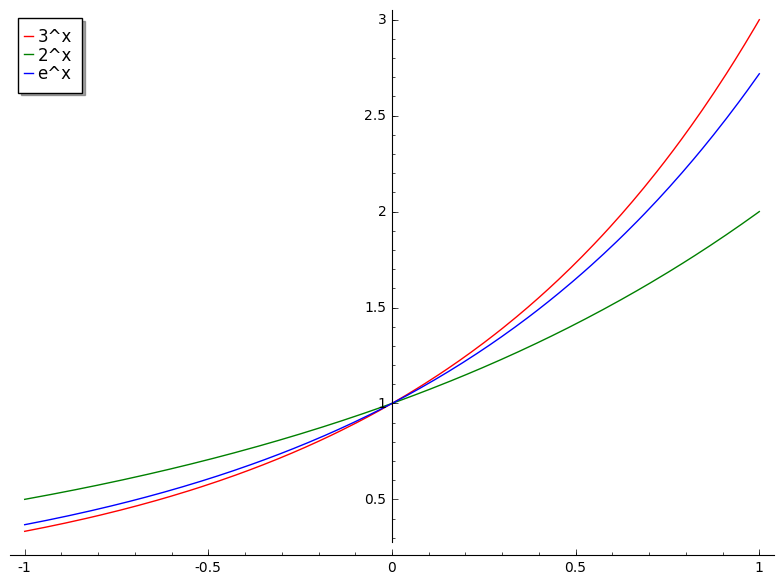
\includegraphics[scale=0.25]{imgs/exponentials1.png}
    \end{center}
    \columnbreak
    \begin{center}
      $0 < a < 1$:
      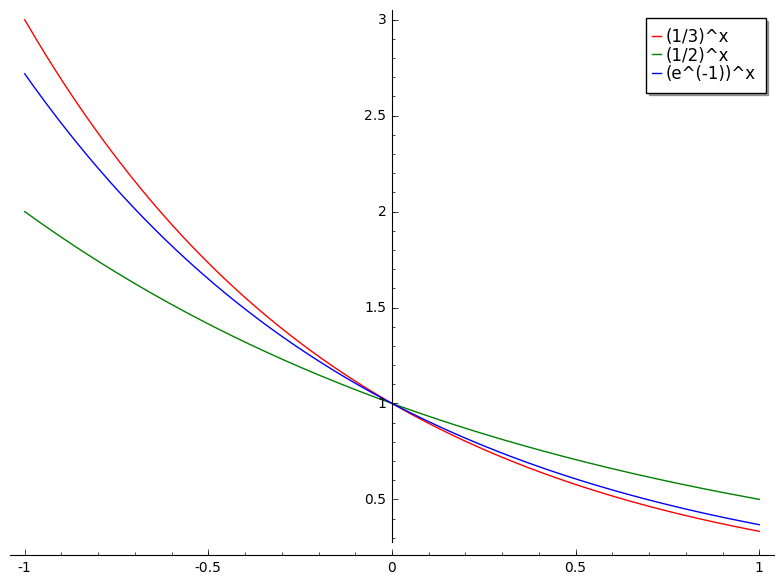
\includegraphics[scale=0.25]{imgs/exponentials2.png}
    \end{center}
  \end{multicols}
\end{frame}

\section{1.6: Logarithms}

\subsection{Inverse Functions}

\begin{frame}{Definition}
  \begin{defn}
    A function $f(x)$ has an {\it inverse} if there exists a function $f^{-1}(x)$ such that
    $$f \circ f^{-1}(x) = x\ \text{and}\ f^{-1} \circ f(x) = x.$$
  \end{defn}
  
  \onslide<2->{
    \begin{thm}[Horizontal Line Test]
      If any horizontal line intersects the graph of $f(x)$ in {\bf at most one} point, then $f(x)$ admits a composition inverse.
    \end{thm}
  }
\end{frame}

\subsection{Definition}

\begin{frame}{Definition}
  First, we note that any exponential function visibly passes the Horizontal Line Test.
  \onslide<2->{
  \begin{defn}
    The {\it logarithm with base a} is the inverse function of the exponential function, $a^x$, and is denoted by
    $$\log_{a}(x).$$
  \end{defn}
  }
  \onslide<3->{
    \begin{rmk}
      \begin{itemize}
      \item<3->
        By definition, 
        $$\log_a(a^x) = x\ \text{and}\ a^{\log_a(x)} = x.$$
      \item<4->
        One denotes $\log_e(x)$ by $\ln(x)$.
      \end{itemize}
    \end{rmk}
    }
\end{frame}

\begin{frame}{Properties of Logarithms}
\begin{itemize}
  \item<1->
    $\log_a(xy) = \log_a(x) + \log_a(y)$
  \item<2->
    $\log_a\left(\frac{x}{y}\right) = \log_a(x) - \log_a(y)$
  \item<3->
    $\log_a\left(x^r\right) = r\log_a(x)$.
  \item<4->
    $\log_a(x) = \frac{\log_b(x)}{\log_b(a)}$.
\end{itemize}
\end{frame}

\begin{frame}{Example}
  Solve $3^t = 10$ for $t$.
  \begin{eqnarray*}
    \onslide<2->{\Rightarrow \ln(3^t) &=& \ln(10)\\}
    \onslide<3->{\Rightarrow t\ln(3) &=& \ln(10)\\}
    \onslide<4->{\Rightarrow t &=& \frac{\ln(10)}{\ln(3)} (= \log_3(10))}
  \end{eqnarray*}
\end{frame}

\begin{frame}{Example}
  Solve $12 = 5e^{3t}$ for $t$.
  \begin{eqnarray*}
    \onslide<2->{\Rightarrow e^{3t} &=& \frac{12}{5}\\}
    \onslide<3->{\Rightarrow \ln(e^{3t}) &=& 3t = \ln\left(\frac{12}{5}\right)\\}
    \onslide<4->{\Rightarrow t &=& \frac{1}{3}\ln\left(\frac{12}{5}\right)}
  \end{eqnarray*}
\end{frame}

\subsection{Exponential Functions with Base $e$}

\begin{frame}
  With the natural logarithm, we can rewrite any exponential function with base $e$ if we so choose.
  \onslide<2->{Say, $P(t) = P_0a^t$.}
  \onslide<3->{We let $k = \ln(a)$ so $e^k = a$ and hence 
    $$P_0e^{kt} = P_0\left(e^k\right)^t \onslide<4->{= P_0a^t} \onslide<5->{ = P(t)}$$}
  \onslide<6->{We call $k$ the {\it continuous growth/decay rate}}.
\end{frame}

\begin{frame}{Example}
  Convert $P(t) = 1000e^{0.05t}$ to the form $P_0a^t$.
  
  \onslide<2->{Let $a = e^{0.05}$.}
  \onslide<3->{Then
    $$P(t) = 1000e^{0.05t} = 1000(e^{0.05})^t = 1000a^t.$$}
\end{frame}

\begin{frame}{Example}
  Convert $P(t) = 500(1.06)^t$ to the form $P_0e^{kt}$.
  
  \onslide<2->{$$P(t) = 500(1.06)^t = 500e^{\ln(1.06)t}.$$}
\end{frame}
\end{document}
